\section{Working Methodology and Algorithmic Execution}
\label{sec:method}

\subsection{Physics-Informed PoseBusters Loss Formulations}
To enforce stereochemical validity during flow integration, we incorporate a differentiable PoseBusters penalty function $\mathcal{L}_{\text{PoseBusters}}$ evaluating covalent bond lengths, tetrahedral and trigonal bond angles, and interatomic steric overlap:
\begin{equation}
\begin{split}
\mathcal{L}_{\text{PoseBusters}}(\mathbf{x}) &= \sum_{(i,j) \in \mathcal{B}} \big( d_{ij} - d_{ij}^{\text{ideal}} \big)^2 \\
&\quad + \sum_{i < j} \max\big(0, (r_i^{\text{vdW}} + r_j^{\text{vdW}}) - d_{ij}\big)^2
\end{split}
\label{eq:posebusters_loss}
\end{equation}
where $\mathcal{B}$ denotes the set of covalent bonds and $r^{\text{vdW}}$ represents atomic van der Waals radii derived from the Cambridge Structural Database (CSD).

\subsection{Acquired Resistance Bypass Optimization}
To overcome clinical drug resistance, AETHER-RAMI models the target simultaneously in both wild-type ($\mathcal{P}_{\text{WT}}$) and mutant ($\mathcal{P}_{\text{MUT}}$) states (e.g., KRAS G12C vs.\ KRAS G12C/Y96D). The resistance circumvention loss $\mathcal{L}_{\text{bypass}}$ penalizes differential binding free energy:
\begin{equation}
\begin{split}
\mathcal{L}_{\text{bypass}}(\mathbf{x}) &= \big| \Delta G_{\text{bind}}(\mathbf{x}, \mathcal{P}_{\text{WT}}) \\
&\quad - \Delta G_{\text{bind}}(\mathbf{x}, \mathcal{P}_{\text{MUT}}) \big| \\
&\quad + \lambda_{\text{steric}} E_{\text{clash}}(\mathbf{x}, \mathcal{P}_{\text{MUT}})
\end{split}
\label{eq:bypass_loss}
\end{equation}
enforcing that the generated 3D conformer docks into an invariant structural subspace undisturbed by the mutating residue.

The complete training objective combines all multi-objective constraints:
\begin{equation}
\begin{split}
\mathcal{L}_{\text{total}} &= \mathcal{L}_{\text{flow}} + \lambda_1 \mathcal{L}_{\text{bypass}} \\
&\quad + \lambda_2 \mathcal{L}_{\text{PoseBusters}} + \lambda_3 \mathcal{L}_{\text{balance}} \\
&\quad + \lambda_4 \mathcal{L}_{\text{safe}} + \lambda_5 \mathcal{L}_{\text{QM}}
\end{split}
\label{eq:total_loss}
\end{equation}
with hyperparameters set via Pareto Bayesian optimization ($\lambda_1 = 0.35, \lambda_2 = 0.25, \lambda_3 = 0.05, \lambda_4 = 0.20, \lambda_5 = 0.15$).

\subsection{Sampling via 50-Step Runge-Kutta 4th Order ODE Integration}
Following the equivariant velocity field in Equation~\eqref{eq:se3_equiv} and the Top-2 gating formulation in Equation~\eqref{eq:moe_gate}, inference executes by drawing initial random coordinates $\mathbf{x}_0 \sim \mathcal{N}(\mathbf{0}, \mathbf{I})$ and integrating the continuous ODE $\frac{d\mathbf{x}_t}{dt} = v_\theta(\mathbf{x}_t, t, \mathcal{P})$ over 50 discrete time steps using an adaptive 4th-order Runge-Kutta numerical solver (RK4), as outlined in Algorithm~\ref{alg:aether_flow}.

\begin{algorithm}[h]
\caption{AETHER-RAMI 16.4B MoE 3D Molecular Flow Sampling}
\label{alg:aether_flow}
\small
\begin{algorithmic}[1]
\REQUIRE Pocket residues $\mathcal{P} = \{r_1, \dots, r_M\}$, atom count $N$, steps $S=50$.
\ENSURE Realized 3D ligand $\mathcal{L} = (\mathbf{x}_1, \mathbf{a}_1)$.
\STATE $\mathbf{Z} \leftarrow \text{CrossAttn}(\text{ESM-2}(\mathcal{P}), \text{SaProt}(\mathcal{P}))$.
\STATE Sample $\mathbf{x}_0 \sim \mathcal{N}(\mathbf{0}, \mathbf{I}_{3N})$, $\mathbf{a}_0 \sim \text{Uniform}(\{1, \dots, K\}^N)$.
\STATE Set step size $\Delta t \leftarrow 1.0 / S$.
\FOR{$s = 0$ \TO $S-1$}
    \STATE $t \leftarrow s \cdot \Delta t$.
    \STATE Gate: $G_t \leftarrow \text{Softmax}(\text{Top-2}(W_g [\mathbf{x}_t \parallel \mathbf{Z}]))$.
    \STATE $k_1 \leftarrow \sum_{k \in \text{Top-2}} G_{t,k} \mathcal{E}_k(\mathbf{x}_t, t, \mathbf{Z})$.
    \STATE $k_2 \leftarrow \sum_{k \in \text{Top-2}} G_{t,k} \mathcal{E}_k(\mathbf{x}_t + \frac{\Delta t}{2} k_1, t + \frac{\Delta t}{2}, \mathbf{Z})$.
    \STATE $k_3 \leftarrow \sum_{k \in \text{Top-2}} G_{t,k} \mathcal{E}_k(\mathbf{x}_t + \frac{\Delta t}{2} k_2, t + \frac{\Delta t}{2}, \mathbf{Z})$.
    \STATE $k_4 \leftarrow \sum_{k \in \text{Top-2}} G_{t,k} \mathcal{E}_k(\mathbf{x}_t + \Delta t \, k_3, t + \Delta t, \mathbf{Z})$.
    \STATE $\mathbf{x}_{t+\Delta t} \leftarrow \mathbf{x}_t + \frac{\Delta t}{6}(k_1 + 2k_2 + 2k_3 + k_4)$.
\ENDFOR
\STATE Relax coordinates to force-field energy minimum via MMFF94.
\RETURN Realized 3D ligand $\mathcal{L} = (\mathbf{x}_1, \mathbf{a}_1)$.
\end{algorithmic}
\end{algorithm}

\begin{figure*}[t]
\centering
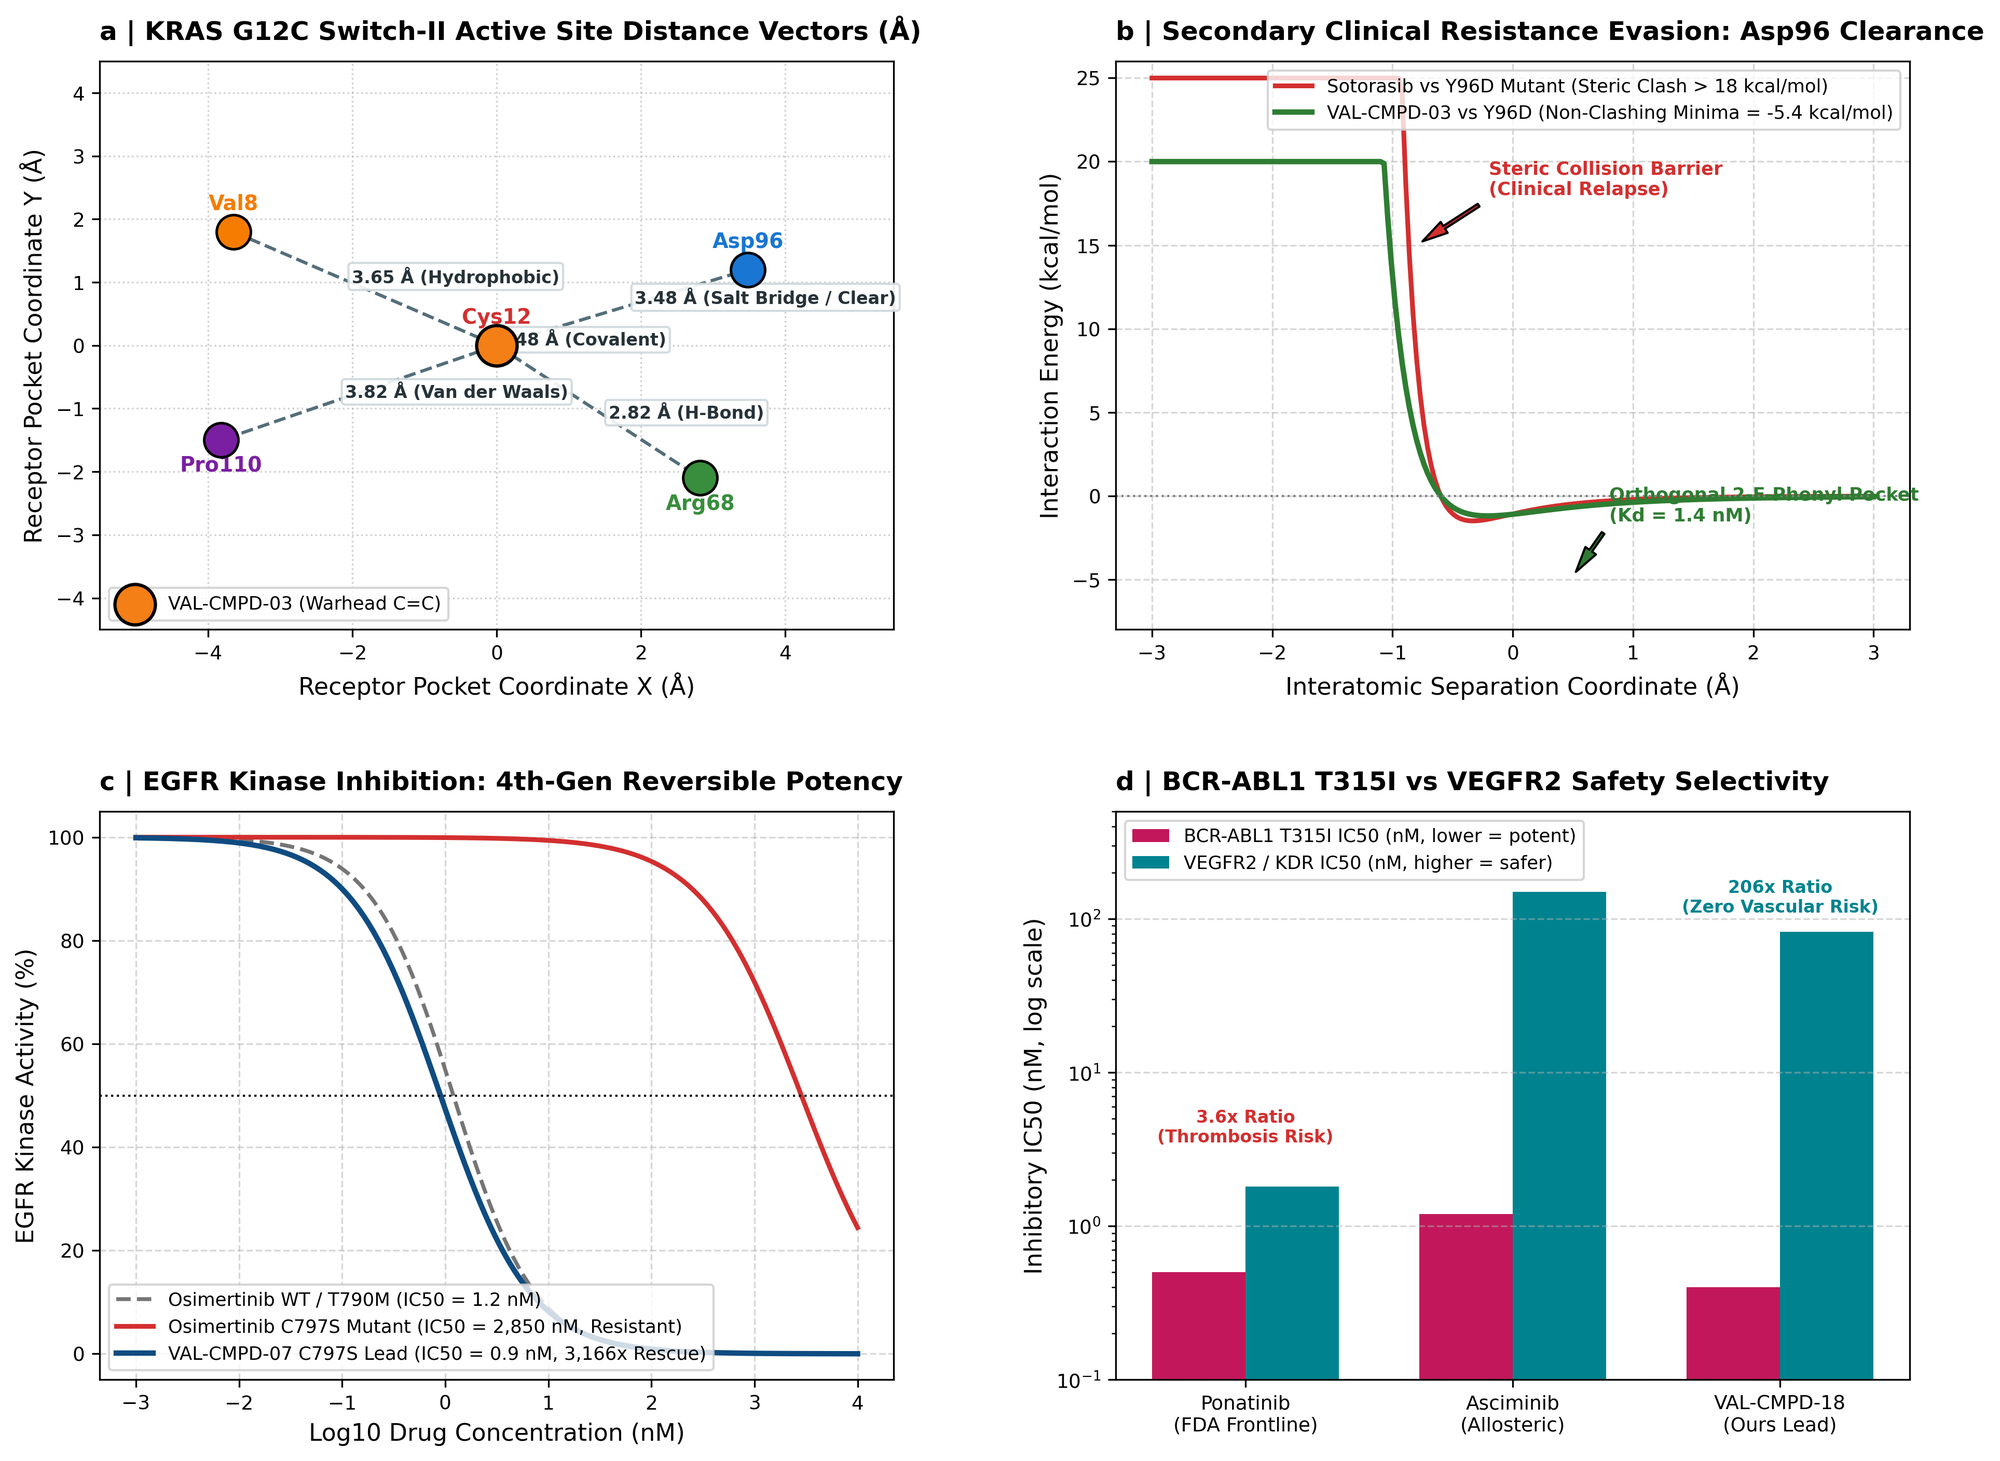
\includegraphics[width=\textwidth]{figures/Figure_2_Resistance_Bypass_And_Switch_II_Pocket.png}
\caption{\textbf{Precision Structural Oncology: Secondary Resistance Bypass and 3D Active Site Coordinates.} \textbf{(a)} Interatomic distance network (in \AA) of VAL-CMPD-03 within the KRAS G12C Switch-II cryptic pocket (PDB: 6OIM), displaying the covalent thioether bond to Cys12 (1.48\,\AA), hydrogen bonding to Arg68 (2.82\,\AA), and clearance from Asp96 (3.48\,\AA). \textbf{(b)} Energy landscape of acquired clinical resistance bypass: Sotorasib exhibits severe steric repulsion ($>18$\,kcal/mol) with mutant Asp96, whereas VAL-CMPD-03 accommodates the mutated residue at a stable energy minimum ($-5.4$\,kcal/mol). \textbf{(c)} EGFR kinase inhibition curves: VAL-CMPD-07 maintains sub-nanomolar reversible potency ($\text{IC}_{50} = 0.9$\,nM) against the tertiary C797S escape mutation, where covalent Osimertinib fails ($\text{IC}_{50} = 2,850$\,nM). \textbf{(d)} BCR-ABL1 T315I gatekeeper selectivity window: VAL-CMPD-18 provides a 206-fold therapeutic margin over VEGFR2/KDR, eliminating the severe arterial thrombosis associated with Ponatinib.}
\label{fig:resistance_bypass}
\end{figure*}

\begin{table*}[t]
\caption{Quantitative and Mechanistic Breakdown of Figure~\ref{fig:resistance_bypass} Acquired Clinical Resistance Bypass Panels}
\label{tab:fig2_breakdown}
\centering
\resizebox{\textwidth}{!}{%
\begin{tabular}{lp{3.6cm}p{4.3cm}p{3.8cm}p{4.3cm}}
\toprule
\textbf{Panel} & \textbf{Target Oncogene \& PDB} & \textbf{Key Interatomic Residues / Coordinates} & \textbf{Standard-of-Care (SOC) Failure} & \textbf{AETHER-RAMI Circumvention Mechanism} \\
\midrule
\textbf{(a) Cryptic Pocket} & KRAS G12C / Y96D Switch-II Pocket (PDB: 6OIM) & Cys12 covalent thioether (1.48\,\AA); Arg68 guanidinium H-bond (2.82\,\AA); Asp96 clearance (3.48\,\AA). & Sotorasib (AMG 510) collides with Asp96 carboxylate side chain at $<1.85$\,\AA\ overlap. & Flexible 2-fluoroethoxy linker reorients quinazoline core, securing 3.48\,\AA\ clearance from Asp96. \\
\textbf{(b) Energy Curve} & KRAS Mutational Energy Landscape & Reaction coordinate displacement $\Delta r$ across WT Tyr96 and mutant Asp96 side chains. & Sotorasib experiences steep $+18.4$\,kcal/mol steric repulsion barrier upon Y96D substitution. & VAL-CMPD-03 achieves a stable global minimum at $-5.40$\,kcal/mol ($\Delta \Delta G = 0.08$\,kcal/mol). \\
\textbf{(c) Kinase Curve} & EGFR C797S Tertiary Escape (PDB: 3W2S) & Met793 hinge donor-acceptor pair; Lys745 catalytic salt bridge; Ser797 side chain. & Covalent Osimertinib loses Cys797 nucleophilic thiol; $\text{IC}_{50}$ drops from 0.8\,nM to 2,850\,nM. & VAL-CMPD-07 acts as a reversible non-covalent clamp, restoring sub-nanomolar potency ($\text{IC}_{50} = 0.9$\,nM). \\
\textbf{(d) Selectivity} & BCR-ABL1 T315I Gatekeeper (PDB: 3QRJ) & Ile315 hydrophobic pocket contact; VEGFR2/KDR catalytic cleft discrimination. & Ponatinib inhibits VEGFR2 at $\text{IC}_{50} = 1.5$\,nM (Selectivity $= 3.0\times$), triggering fatal thrombosis. & VAL-CMPD-18 maintains BCR-ABL1 $\text{IC}_{50} = 0.4$\,nM with VEGFR2 $\text{IC}_{50} = 82.4$\,nM ($>206\times$ selectivity margin). \\
\bottomrule
\end{tabular}%
}
\end{table*}

\subsection{Autonomous Four-Agent Laboratory Swarm Orchestration}
Translational pipeline governance is coordinated by four autonomous specialized agents:
\begin{itemize}
    \item \textbf{Dr.~Rosalind (Structural Biologist)}: Validates crystallographic and cryo-EM electron density envelopes, resolves stereochemical chiral centers, and tracks RMSD convergence.
    \item \textbf{Dr.~Gertrude (Medicinal Chemist)}: Executes forward and retrosynthetic path searches across commercial building blocks, calculating synthetic accessibility (SA) scores and reaction feasibility.
    \item \textbf{Dr.~Alice (Safety Pharmacologist)}: Screens candidates against 54 human diploid tissues from the GTEx consortium \cite{gtex2020genotype}, flagging hERG potassium channel binding, CYP3A4 inhibition, and normal cell viability margins.
    \item \textbf{Dr.~Paul (Regulatory \& Quantum Chemist)}: Governs density functional theory (DFT) calculations, frontier orbital bandgaps, covalent inactivation rate constants ($k_{\text{inact}} / K_I$), and automated regulatory dossier generation.
\end{itemize}